\scanpage{71}
\[
\bigotimes_{i\in K}L_i=L_K
\]
\deleted{$\unsure{A}$}
\figure{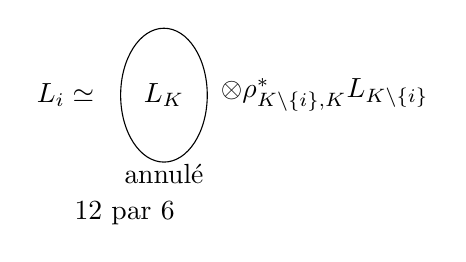
\begin{tikzpicture}[every node/.style={font=\normalsize}]
\node at(0,0){$L_i\simeq$};\node at(1.25,0){$\uline{L_K}$};\draw(1.25,0)ellipse(.55 and .85);
\node[anchor=west]at(1.85,0){$\otimes\rho_{K\setminus\{i\},K}^{*}L_{K\setminus\{i\}}$};
\node at(1.25,-1){annulé};\node at(.75,-1.5){\deleted{$12$ \unsure{par} $6$}};
\end{tikzpicture}}
\diagram{\begin{array}{l|c|c|c}
n&4&5&6\\\hline
(n-1)(n-2)&6&12&20\\\hline
\begin{gathered}\text{meilleur}\\\text{\unsure{exposant}}\\\text{pour trivialiser}\\L\end{gathered}&3&12?&20?\\\hline
\begin{gathered}\text{meilleur}\\\text{\unsure{exp.} pour}\\\text{trivialiser }L_i\end{gathered}&6&12?&60?\\\hline
\begin{gathered}\text{exposant}\\\text{pour}\\\text{trivialiser}\\\uuline{H^1(M_{0,I},\mathfrak S_I;\mathbb G_m)}\end{gathered}&&&\\\hline
\begin{gathered}\text{\unsure{diviseurs}}\\H^1(M_{0,I},\mathfrak S_{I\setminus\{i\}};\mathbb G_m)\end{gathered}&&&\\\hline
\end{array}}
\figure{\begin{tikzpicture}\draw(0,0)--(2,.9);\end{tikzpicture}}
\[
L_K\qquad\text{cas }n=5
\]
\[
\unsure{\simeq}\prod_{A\in\mathcal P_4}\rho_A^*(\uline{L_A})
\]
\inserted{annulé par $3$}
\[
=\prod_{\substack{\unsure{(i,A)|(i\in A)}\\i\in A\in\mathcal P_4(K)}}L_i
=\left(\prod_{i\in K}L_i\right)^{\otimes4}
=L^4
\]
\[
(L^4)^3\simeq\mathcal O
\]
\deleted{\unsure{annulé par}}

\figure{
\begin{tikzpicture}
\node[yscale=-1,transform shape,text=gray,inner sep=0pt]{\begin{minipage}{12.5cm}\scriptsize
\unsure{UNIVERSITE DES SCIENCES ET TECHNIQUES}\hfill\unsure{Montpellier, le}\ \illegible{2}\ \unsure{1979}\\
\unsure{DU LANGUEDOC}\\
\uline{\unsure{MONTPELLIER}}\\[12pt]
\hspace*{3cm}\unsure{C.}\ \illegible{4}\\
\hspace*{3cm}\uline{\unsure{Section de la Physique}}\\[18pt]
\illegible{14}\\
\illegible{18}\\
\illegible{2}\ \unsure{de l'Université}\\[5pt]
\illegible{2}
\end{minipage}};
\end{tikzpicture}}
\mspage{70}
